
%\section{Calibration and Validation}
%\section{Validation}
\label{sec:validation}

% VALIDATION TODO
%
% show major effort
% table of results
% show hierarchy
% precisely define cases 
%
%

%
% meshed vanes are 24x more expensive
%

The previous sections briefly outlined the physical phenomenon under
consideration, the mathematical models proposed to simulate it,
and the numerical solution of these models for a variety of system 
configurations and scenarios. Before these simulations can be used 
as a tool to evaluate proposed system designs, it is necessary to
validate that the physical model in use accurately represent
reality. This section contains a discussion of the validation of the
computational models against existing experimental data and high
fidelity simulations. 

A challenge in this project is the scarcity of experimental data. Only
two or three cases of experimental measurements are available. These
measurements, for reasons detailed in the next subsection, are not
sufficient to provide confidence in the output of simulations across a
wide variety  of scenarios. Therefore, a high fidelity model using 
meshed vanes with enforced no-slip velocity boundary conditions along
the surface of the vane was developed. These ``gridded'' runs have
been validated against the experimental data, which they match quite
closely. However, as detailed in Section~\ref{subsec:vane}, 
explicitly meshing the vanes would be far too 
prohibitively expensive to permit a rapid exploration of a variety of
system configurations. Instead, this high fidelity model is used 
to generate additional reliable data to permit validation of lower
fidelity models, such as the virtual vanes. Likewise, the results of the
unsteady virtual vane simulations can be used as validation data for a
further reduced, steady Navier-Stokes model. This hierarchy of
validation is shown in Figure~\ref{fig:val_hier}, with data sources that
generate more reliable data at the top, and models that are less
reliable, but also less computationally expensive at the bottom. In
terms of expense, the steady virtual vane model generates a solution in
approximately two minutes, versus twelve hours for the unsteady virtual
vane model. The gridded vanes require another factor of ten in
computational time, and many more man-hours hours of work to generate
the mesh. Therefore, it is unrealistic to perform parameter sweeps or
system configuration investigations with the gridded vanes and these
results are used only for validation studies. Instead, the
ROM is used, with promising results re-evaluated with unsteady virtual
vane models. %and so on up the hierarchy if more confidence is necessary. 

%
% https://www.draw.io/
%
 \begin{figure}[!htb]
   \begin{center}
    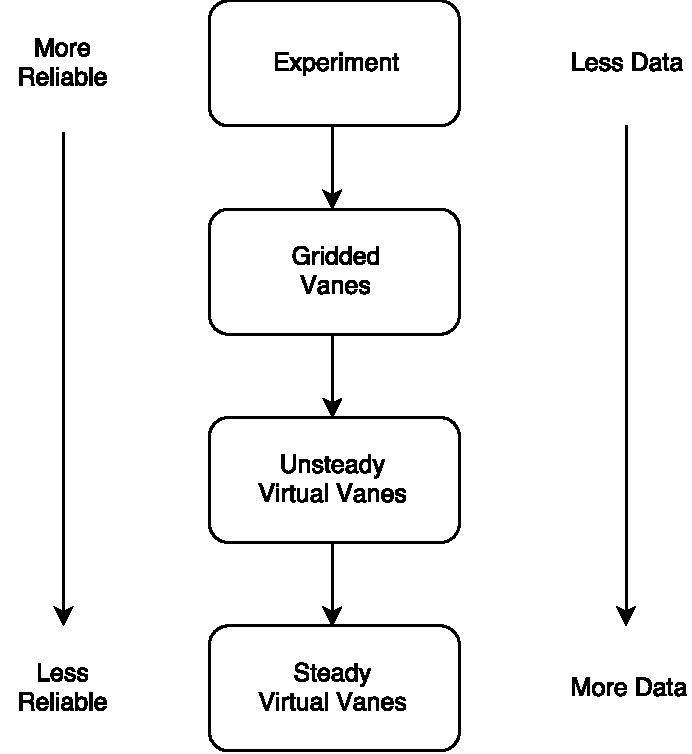
\includegraphics[width = 8 cm]{figs/validation_hierarchy}
    \caption{This figures depicts the validation hierarchy. The
    experimental measurements 
    are at the top, where the data is expected to be the most reliable,
    but simultaneously the most limited. Moving down the table leads to
    simulated data sources that are less reliable but increasingly
    cheaper in time to generate. At the bottom is the reduced order
    model from steady virtual vane solutions.} 
    \label{fig:val_hier}
   \end{center}
 \end{figure}

Three kinds of experimental validation data are available. These are
data generated in the laboratory using a heated plate, data from
experiments in the wind tunnel (``Wind-only''), and measurements from field
tests (``Field'') conducted in Arizona. The available data from
these cases as well as the gridded vanes created to mimic them are are
summarized in Table~\ref{tab:val_data}. Every case shown has been
simulated using the virtual vanes.   

%\large
\begin{table}[h]
\centering
\label{my-label}
\begin{tabular}{l|l|l|l|}
           & Wind-Only                   & Thermal-Only                & Field  \\
  \hline 
Experiment & Straight Vanes $60^{\circ}$ & Straight Vanes $60^{\circ}$ & June 2014   \\
           &                           & Straight Vanes $30^{\circ}$   & August 2014 \\
           &                           & Hybrid (Two tier)             & August 2015 \\
  \hline 
Gridded    & Straight Vanes $60^{\circ}$ & Straight Vanes $60^{\circ}$ & \\
           & Straight Vanes $30^{\circ}$ & Straight Vanes $30^{\circ}$ & \\
  \hline 
\end{tabular}
  \caption{Available truth data from the laboratory experiments 
    (cold wind and thermal-only), the field test, and the gridded vanes.} 
  \label{tab:val_data}
\end{table}
%
%
%
% http://www.tablesgenerator.com/
%
%

%
% experimental challenges
%
%\normalsize
\subsection{Thermal-Only Validation}
This section provides examples of the validation performed with the
richest data set, the measurements in the laboratory. All of the
thermal-only the data was generated in a laboratory setting at Georgia
Tech. The general system configuration is depicted in Figure
\ref{fig:lab_image}. These data were taken using particle image
velocimetery (PIV), and the errors in in measurement and sampling are
not known. In addition, only velocity measurements are
available. Several potentially important quantities of interest, such as
the pressure and temperature, have not been measured. 

%
% http://convertonlinefree.com/ConvertImageEN.aspx
%
 \begin{figure}[!htb]
   \begin{center}
    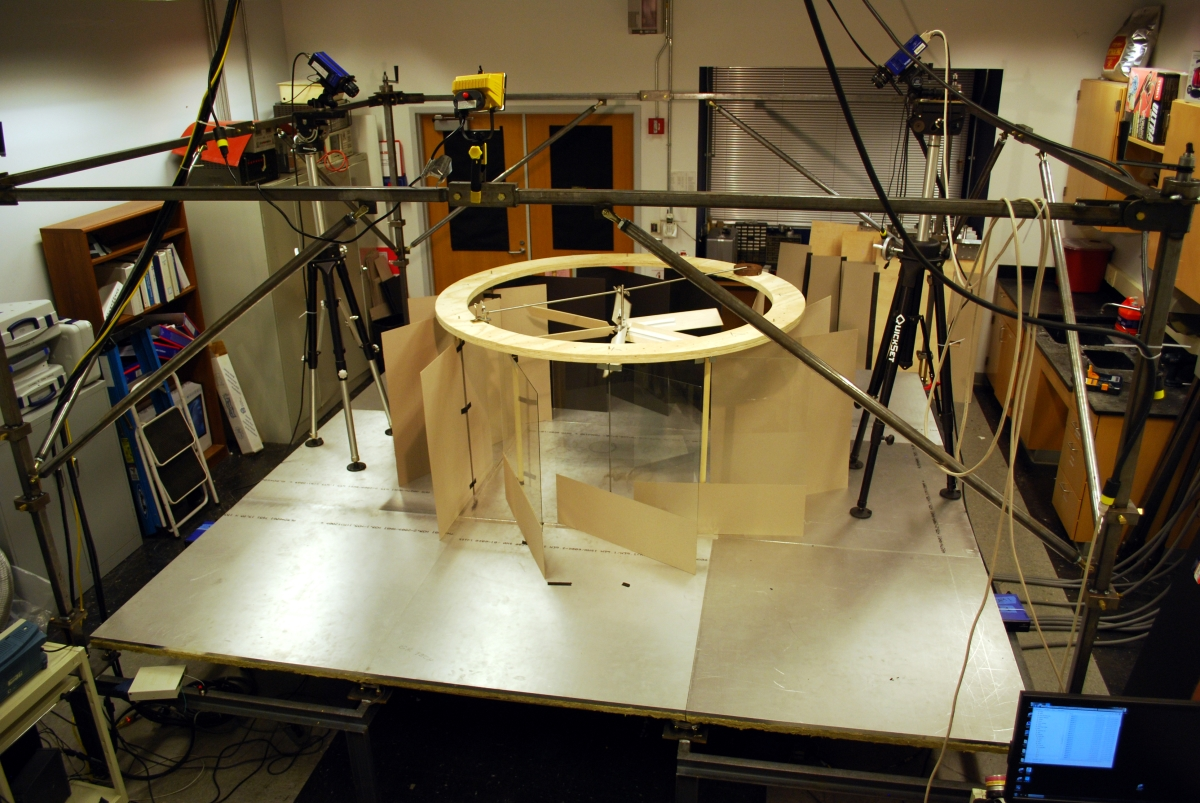
\includegraphics[width = 12 cm]{figs/Optimized-lab_setup}
    \caption{The single tier straight vane laboratory configuration. The
    apparatus is shown with a turbine, but that was removed for data
    gathering.}
    \label{fig:lab_image}
   \end{center}
 \end{figure}

While no sensitivity analysis has been performed, it is likely that the
largest uncertainty in the laboratory simulation is a result of the
ventilation of the laboratory. The heated plate at the bottom of the apparatus
generates enough heat to cause a significant increase in room
temperature (30+ Kelvin), which greatly impacts the SoV
performance, as the ground to air thermal gradient drives the
vortex. The laboratory is cooled to maintain
temperature by two inlet HVAC ducts into the room. 
%While efforts have been made to characterize the level of ventilation being
%used, these numbers come with non-trivial uncertainties attached. 
One vent continuously provides air at 288 Kelvin with a flow rate estimated 
to be 1 $\text{m}^3$/s.
%(4-6 m/s with an approximate area of 0.2 $m^2$)
The other vent is active only if the room temperature exceeds 301 Kelvin, 
with a flow rate also estimated at 1 $\text{m}^3$/s.
Finally, the air leaves through the cracks around the laboratory doors and 
exhaust vents. Preliminary results indicated that an inflow rate of 1
$\text{m}^3$/s, the lower bound of the possible inflow rates results in
excessive heating of the room, while inflow conditions at the maximum
inflow rate of 2 $\text{m}^3$/s result in a simulated room that is too cold,
compared to the laboratory.  

Our simulated vortices are sensitive to ambient room temperature and thus 
the inflow rate. It is likely that the laboratory is run where one of
the vents is operating intermittently. 
To mimic these conditions in our simulations, Dirichlet boundary conditions 
on parts of the sides of the computational domain are used to
establish a constant inflow of cool air at the rates 
proscribed by our collaborators. Over the remainder of the side walls, 
adiabatic thermal boundary conditions are are used. 

The most signficant boundary condition disparity is that flow leaves the
domain through the top boundary, instead of out of the sides of the
room. Preliminary results suggested that the SoV phenomenon  was not
sensistive to these boundary condition details. The important element is
the  global energy balance in the room. The flow rate into the room is
adjusted to  1.3 $m^3$/s for the validation results discussed here.  

%% \begin{figure}[!htb]
%%   \begin{center}
%%    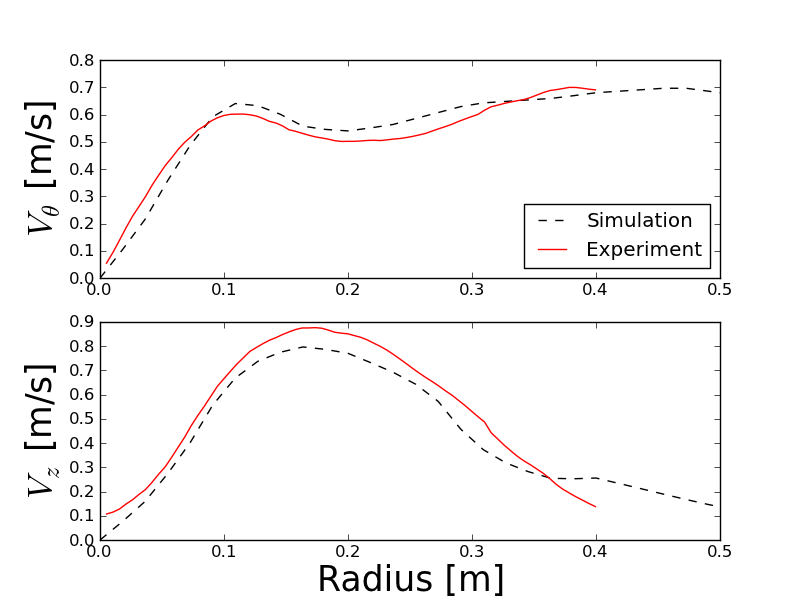
\includegraphics[width = 12 cm]{figs/hybrid_profile}
%%    \caption{Azimuthal and vertical velocity profiles as a function of
%%    radius. The simulation and experimental data broadly agree, with
%%    the simulation also exhibiting the characteristic ``twin-peak''
%%    structure of the hybrid vanes in the azimuthal velocity. }
%%    \label{fig:lab}
%%   \end{center}
%% \end{figure}

\todo{fix me}
% \begin{figure}[htp!]

%  \begin{subfigure}{.5\textwidth}
%   \centering
%   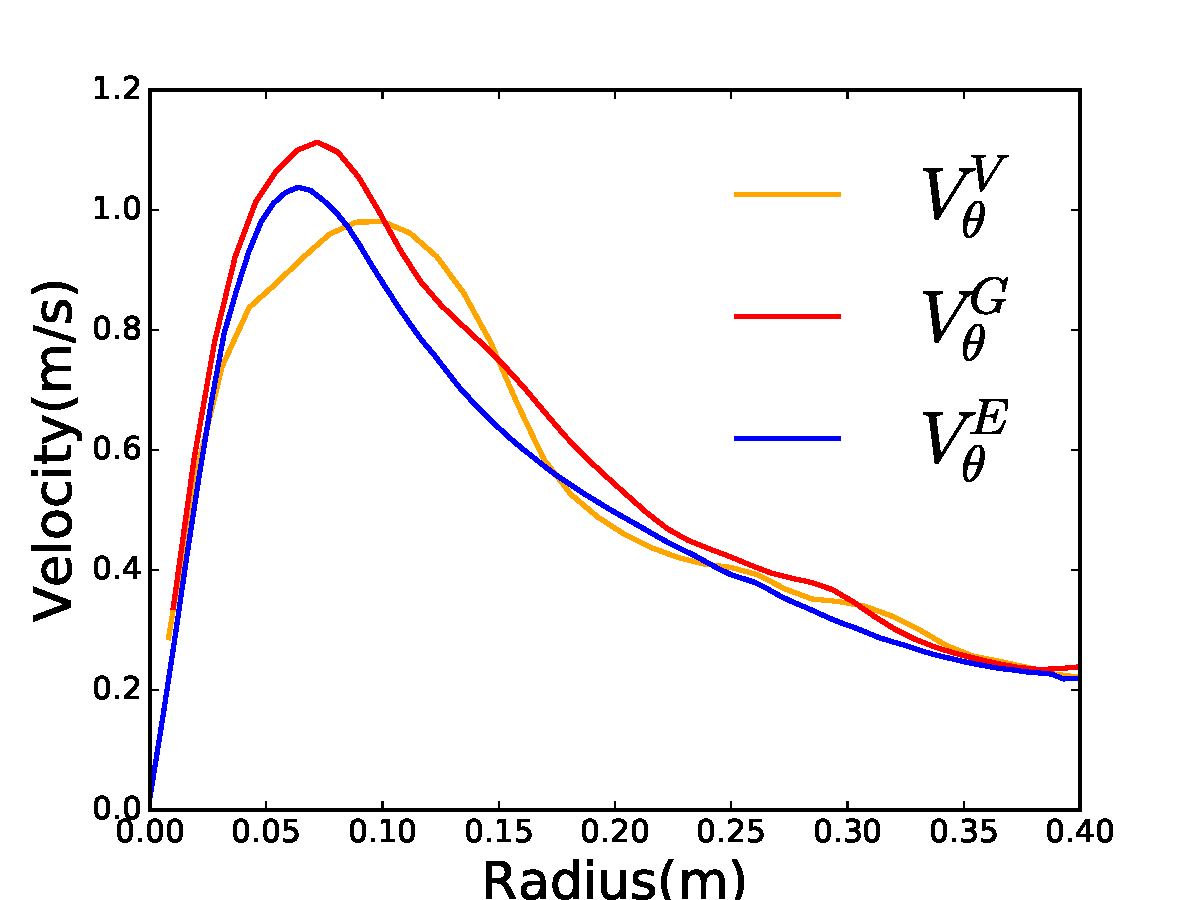
\includegraphics[width =0.9\textwidth]{figs/sim_vs_exp_30_vt}
%   \caption{Azimuthal velocity}
%  \end{subfigure}%
%  \begin{subfigure}{.5\textwidth}
%   \centering
%   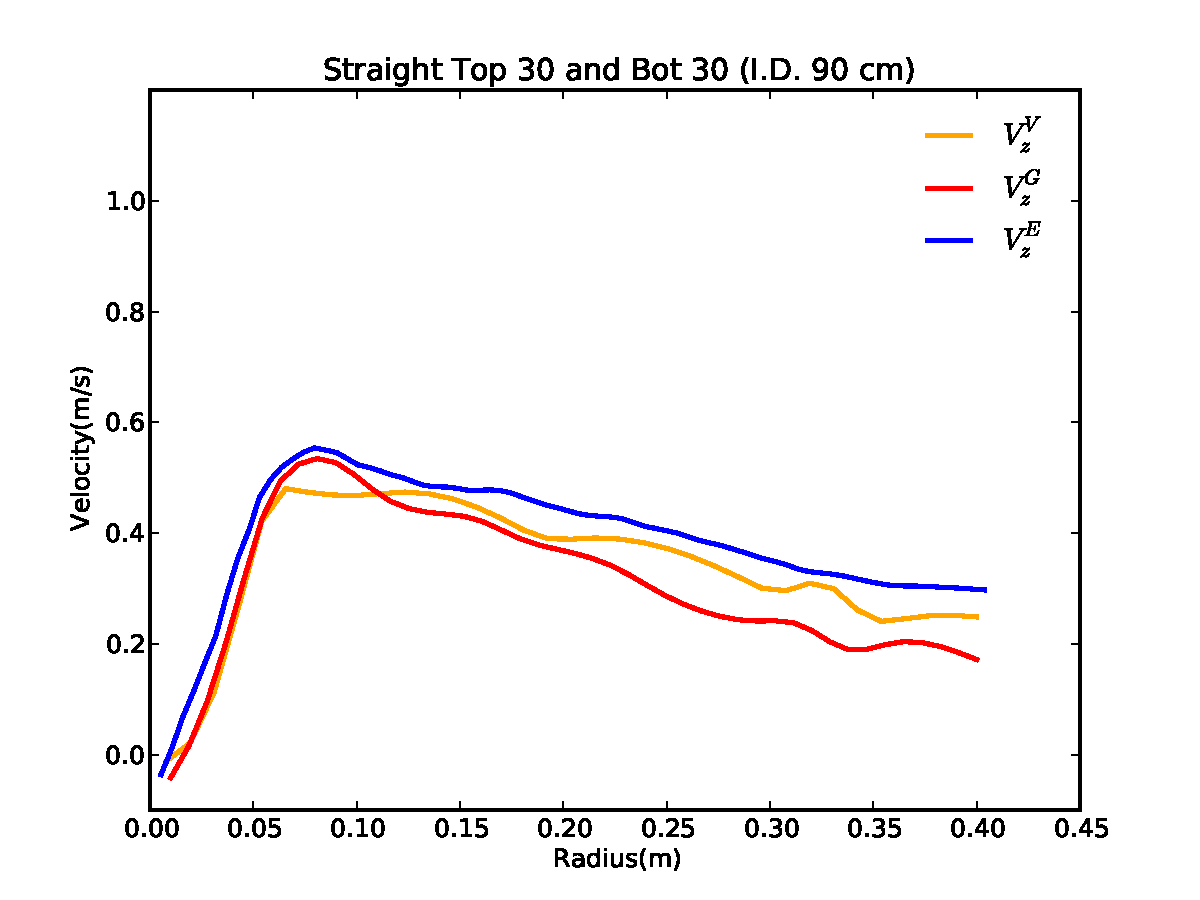
\includegraphics[width =0.9\textwidth]{figs/sim_vs_exp_30_vz}%
%   \caption{Vertical velocity} 
%  \end{subfigure}%
%   \caption{Azimuthal (left) and vertical (right) velocity 
%  as a function of radius for the thermal-only cases. The gold line is
%  the virtual vane simulation, blue the experiment, and red the gridded vane.} 
%   \label{fig:val_lab}  
% \end{figure}

Figure \ref{fig:val_lab} is a direct comparison between laboratory 
measurements for a simple single tier vane configuration ($30^{\circ}$
straight vanes) and nominally identical simulations with the gridded and
virtual vanes. The simulations and experiment broadly agree. The
simulation correctly reproduce the peak structure in the azimuthal
velocity observed for this configuration in the experiment. The gridded
vanes closely represent the peaks radial location, while the
virtual vanes over-predict the radial location. The radial location of
peak vertical velocity also closely agrees with experiment.

Similar validation comparisons have been made between several other
configurations with similar levels of agreement,  notably the
$60^{\circ}$ single tier straight vane case, and the two tier hybrid
vane.  Finally, estimates of the energy fluxes between the field
configuration and our simulation results agreed within 15\%. These
validation studies have provided a level of confidence that our
simulations accurately reproduce the phenomena observed in laboratory.

\subsection{Wind Cases}

The laboratory thermal vortex experiments described in the previous
subsection did not include the effects of the wind, but experience in
the field indicated how important these effects were. To ensure that the
virtual vanes could represent this effect, a validation study 
was performed using the data obtained in the wind tunnel.

A numerical experiment was performed in which the 60 degree single tier
straight vanes were placed in a isothermal wind.  These results were
compared to an identical configuration placed in a wind tunnel.
However, no measurements (of velocity or any quantity) were made
for the vanes in these conditions. Qualitative comparisons, based on
descriptions of observed structures and videos of smoke visualization
were made between the simulations and the wind tunnel experiments. These
images and discussions did not 
identify any inconsistencies between simulation and experiment.
However, these results are limited, and are only for the cold wind, as
the wind tunnel did not include a heated plate.  

% \begin{figure}[htb]

%  \begin{subfigure}{.5\textwidth}
%   \centering
%   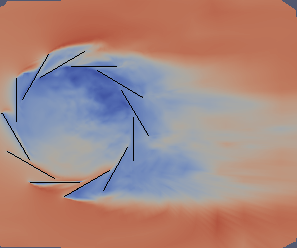
\includegraphics[width=.75\linewidth]{figs/gridded_wind}
%   \caption{Streamwise Velocity: Gridded Vanes}
%  \end{subfigure}%
%  \begin{subfigure}{.5\textwidth}
%   \centering
%   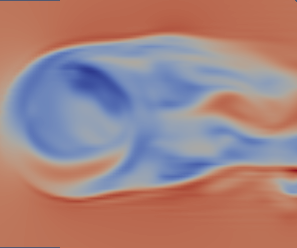
\includegraphics[width=.75\linewidth]{figs/virtual_wind}
%   \caption{Streamwise Velocity: Virtual Vanes}
%  \end{subfigure}%


%  \begin{subfigure}{.5\textwidth}
%   \centering
%   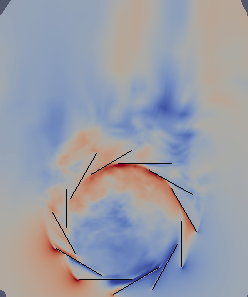
\includegraphics[width=.75\linewidth]{figs/gridded_wind_span}
%   \caption{Spanwise Velocity: Gridded Vanes}
%  \end{subfigure}%
%  \begin{subfigure}{.5\textwidth}
%   \centering
%   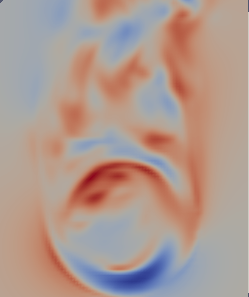
\includegraphics[width=.75\linewidth]{figs/virtual_wind_span}
%   \caption{Spanwise Velocity: Virtual Vanes}
%  \end{subfigure}%

%  \caption{Horizontal slices through the top of the vanes for the
%  wind validation cases. On the left are the explicitly gridded vanes,
%  and on the right the virtual vanes. The streamwise velocity shows
%  penetration through the region where the vanes are aligned with the
%  flow in both the gridded as well as virtual vanes. In addition, the
%  virtual vane case correctly reproduces the direction and magnitude of
%  the spanwise velocity inside the vanes. Finally, the wake has similar
%  structure between the two cases.}
%  \label{fig:wind_val}
% \end{figure}

Figure~\ref{fig:wind_val} contains images of the simulated averaged
streamwise and  spanwise velocity in a horizontal plane at approximately
the height of the vanes obtained from simulations with gridded and
virtual vanes. As expected, there are some differences in the
details of these simulations, but the overall character of the flow
inside the vanes, and in the wake of the vanes is quite similar. This
demonstrates that the virtual vane formulation can indeed represent the
interaction with the wind. 

\subsection{Field Configurations}

Several field tests have been performed by the experimental team. After
each field test, qualitative observations, measurements and lessons
learned are provided by the field team. Actual measurements
are limited. Due to the complexity of the configuration
(two vane tiers and a cone) Gridded vanes cases have not been developed
for the field. This subsection provides a discussion of some of
the results from the latest field test, as an example of typical
validations performed. 

 \begin{figure}[!htb]
  \begin{center}
   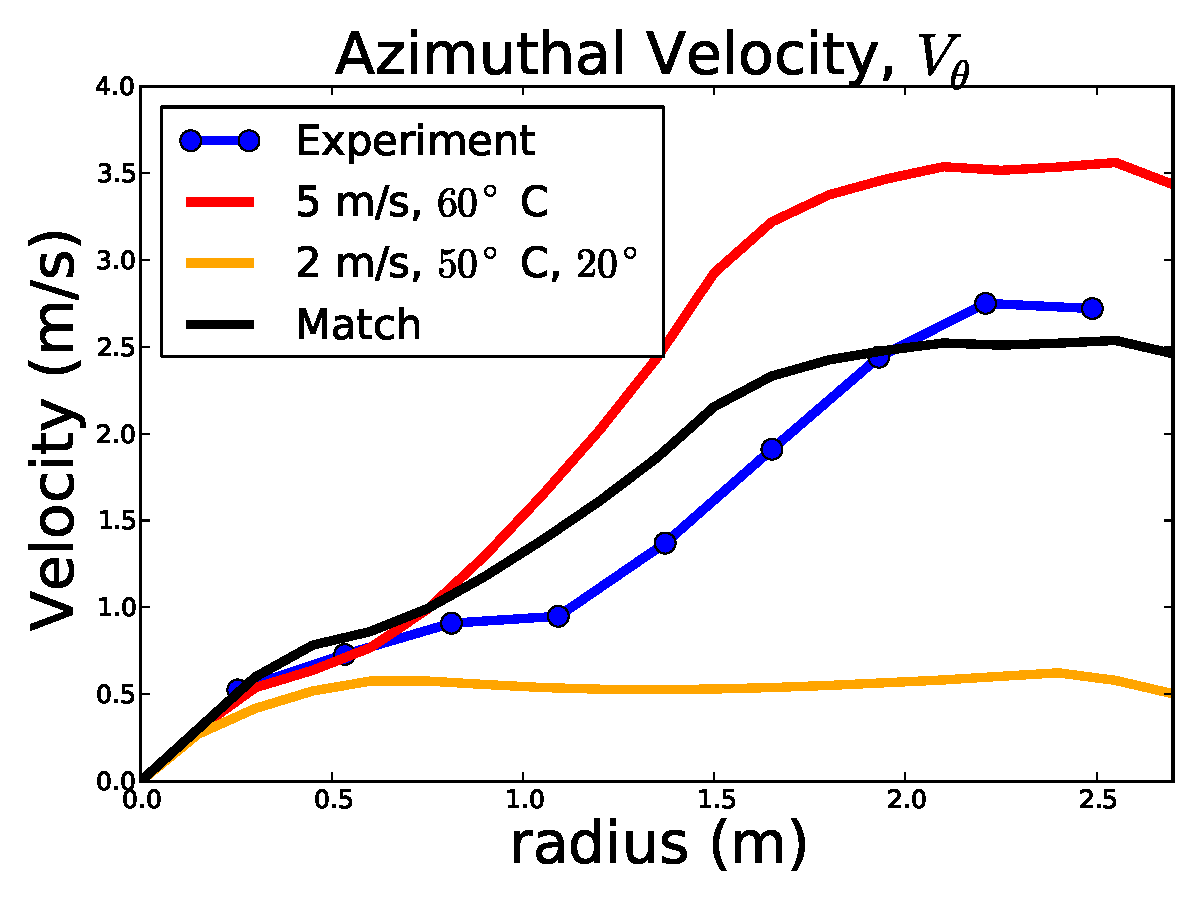
\includegraphics[width = 12 cm]{figs/validate_field}
   \caption{Azimuthal velocity data from the August 2015 field test is
   shown in blue. Two virtual vane simulations with different scenario
   parameters are shown in red and gold. The velocity field was
   temporally averaged but not averaged in space, to reproduce
   the measurements from the field.}
   \label{fig:field_val}
  \end{center}
 \end{figure}
%
% provide an example of these validations below
%

Figure~\ref{fig:field_val} shows data from the August 2015 field test in
blue. These results were obtained using an anonmometer at fixed
azimithal location (believed to be a ninety degree angle, where the zero
is defined to be aligned with the streamwise flow direction) to measure the
azimuthal velocity. The ultrasonic 
anemometer malfunctioned, and the temperature was only measuered at one
location at 1 meter height. A time series from approximately an hour was
gathered. This data included large scenario uncertainties, with
estimated 3 m/s variations in wind, 20 degree wind heading changes, and
10 degree Celsius shifts in temperature. A solidworks CAD file provided
by the experimental team defined the vane and cone
geometry, which were then represented in the simulations as virtual
vanes and a solid surface, as described in 
Sections~\ref{subsec:vane} and~\ref{subsec:solid_surface}.   

To span the range of conditions, several simulations were conducted
with different scenario parameters. The azimuthal velocity from two such
simulations (Red and Gold lines) are plotted against the experimental
data (blue line) in Figure~\ref{fig:field_val}.  

These simulations accurately bound the experimental data. Furthermore, a
``Matching'' case was identified that is broadly consistent with the
field results. The kinetic energy flux, measured in a horizontal plane
at the top of the vanes (where a turbine to extract this energy would
likely be placed), in the simulations agrees with the experimental
estimate within 10\%. 


%
% validation story is incomplete
% 
% you have done: 
%
% 1) comparions between laboratory + gridded + virtual 
% 
% 2) comparisons between gridded + virtual in laboratory
%    + field configurations, thermal only and wind
%
% 3) comparisons of virtual vanes to field observations 
%    quantitative + qualitative
%
%
% You need to discuss what needs to be validated -- the
% comparison to gridded vanes is a useful validation tool 
%
